\documentclass{beamer}

\usepackage{svg}

\usetheme{Boadilla}

% Title
\title{A Brief History of Linux}
\subtitle{Linux Week \the\year{}}
\date{\today}
\institute{Linux Users Group @ UIC}

\begin{document}
\begin{frame}
	\titlepage\footnotetext{Slides adapted from Cody Hasty 2021}
\end{frame}

\begin{frame}{Table of Contents}
	\tableofcontents[pausesections]
\end{frame}

\section{Origin of UNIX}
\subsection{1969-1980}
\begin{frame}{Origin of UNIX}
	\begin{columns}
		\begin{column}{0.5\textwidth}
			\pause
			\begin{figure}
				\centering
				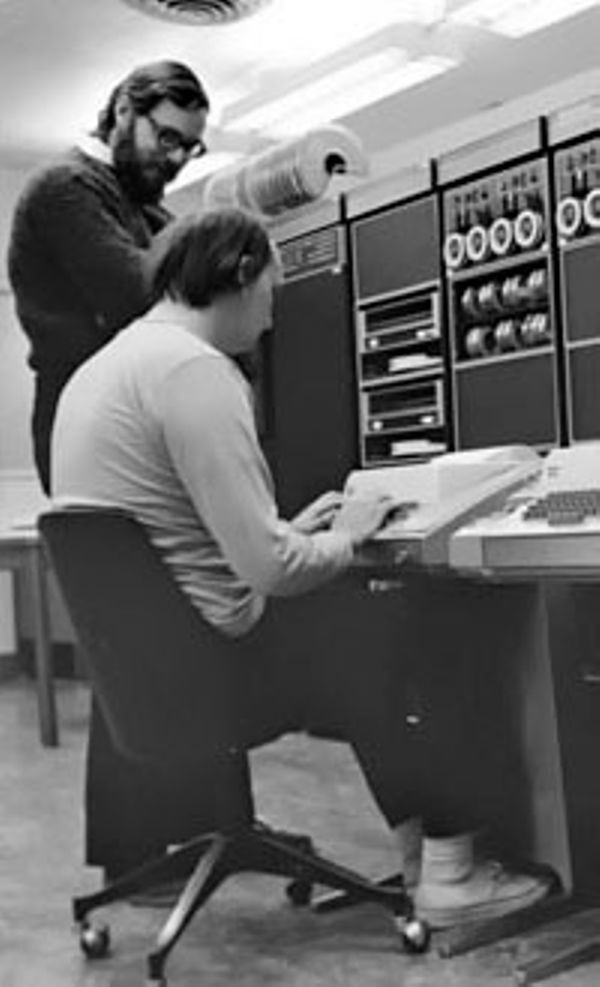
\includegraphics[width=0.50\textwidth]{04february-1.jpg}
				\caption{Ken Thompson (sitting) and Dennis
				Ritchie (standing) in front of a PDP-11 in
				1972.}
			\end{figure}
		\end{column}
		\begin{column}{0.5\textwidth}
			\begin{itemize}
				\item Simplification of a much larger project,
					and the philosophy/community that came
					out of it 1973
					\pause
				\item In 1973, C is invented, UNIX is written
					in it
					\pause
					\begin{itemize}
						\item Allows for compilation on
							machines other than
							PDP-7
					\end{itemize}
					\pause
				\item Unix published in ACM journal, began to
					spread across the world
					\pause
				\item Only universities, corps, etc had
					access/exposure to computing at this
					time
			\end{itemize}
		\end{column}
	\end{columns}
\end{frame}

\begin{frame}{Origin of UNIX}
	\begin{columns}
		\begin{column}{0.5\textwidth}
			\begin{figure}
				\centering
				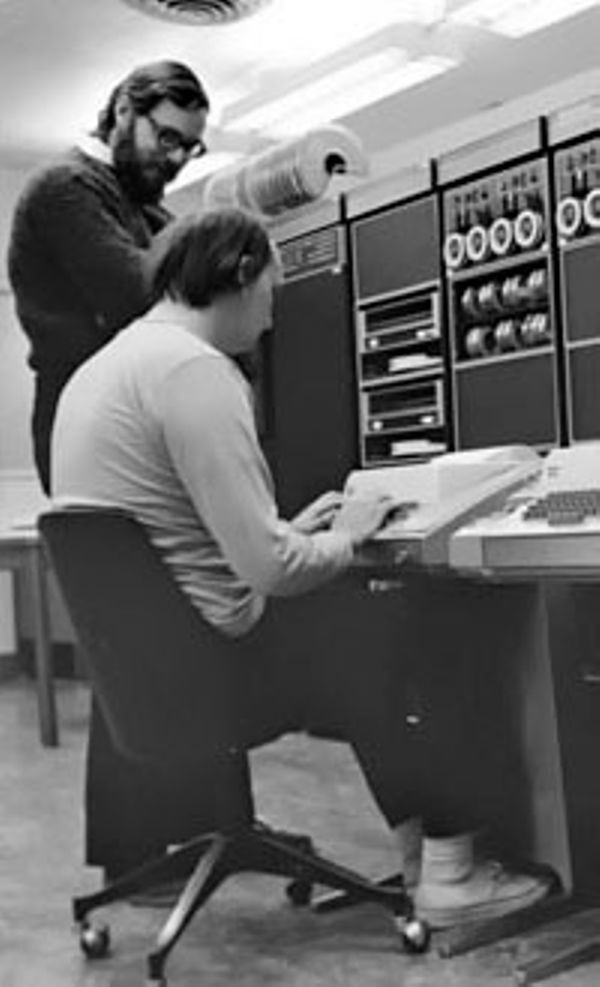
\includegraphics[width=0.50\textwidth]{04february-1.jpg}
				\caption{Ken Thompson (sitting) and Dennis
				Ritchie (standing) in front of a PDP-11 in
				1972.}
			\end{figure}
		\end{column}
		\begin{column}{0.5\textwidth}
			\begin{itemize}
				\item Emergence of counter-culture across
					Universities
					\pause
					\begin{itemize}
						\item Scraggly-haired hippies
							sticking it to the man
							by taking it apart and
							putting it back
							together, together
							Different departments
							created new
							functionalities to
							address the problems of
							their labs
							\pause
						\item Beginning of commercial
							C/Unix tech Massive
							collaboration effort
							due to anti-trust case
							with Bell Labs Couldn’t
							be sold, so the
							creators shipped it to
							anyone who asked for it
							“With Love...Ken”
					\end{itemize}
			\end{itemize}
		\end{column}
	\end{columns}
\end{frame}

\begin{frame}{Origin of UNIX}
	\begin{columns}
		\begin{column}{0.5\textwidth}
			\begin{figure}
				\centering
				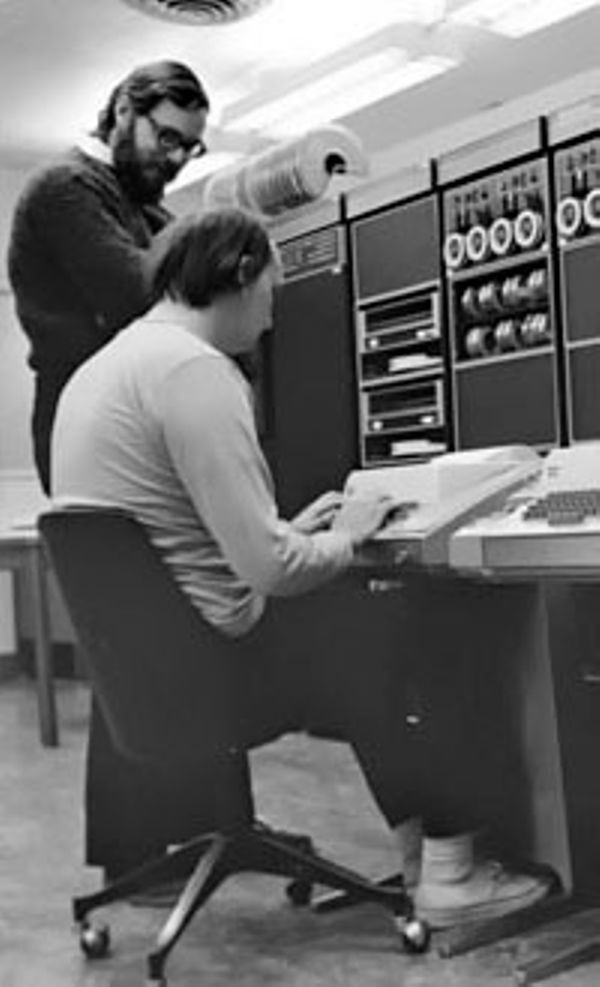
\includegraphics[width=0.50\textwidth]{04february-1.jpg}
				\caption{Ken Thompson (sitting) and Dennis
				Ritchie (standing) in front of a PDP-11 in
				1972.}
			\end{figure}
		\end{column}
		\begin{column}{0.5\textwidth}
			\begin{itemize}
				\item UNIX Version 7 in 1979: Not the first
					computer, but the first system you and
					I would look at and look at and say
					‘that’s a computer’
			\end{itemize}
		\end{column}
	\end{columns}
\end{frame}

\section{Origin of the Internet}
\subsection{1969-1980}
\begin{frame}{Origin of the Internet}
	\begin{columns}
		\begin{column}{0.5\textwidth}
			\begin{figure}
				\centering
				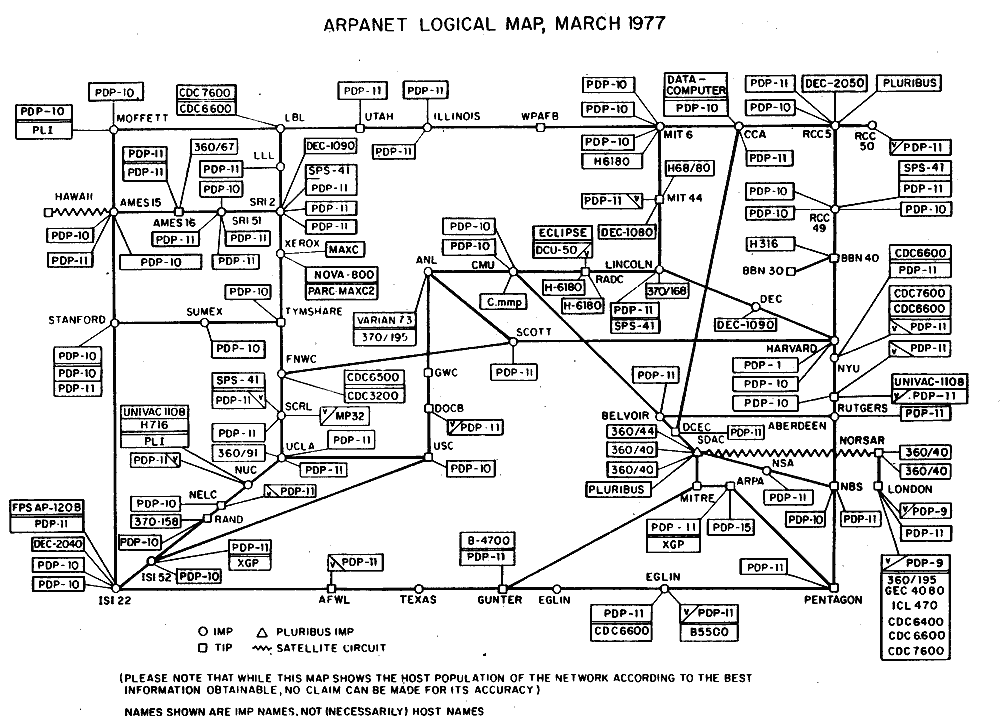
\includegraphics[width=\textwidth]{Arpanet_logical_map,_march_1977.png}
				\caption{ARPANET logical map circa 1977}
			\end{figure}
		\end{column}
		\begin{column}{0.5\textwidth}
			\begin{itemize}
				\item 1969 - ARPANET
					\pause
				\item Did NOT use UNIX
					\pause
				\item MIT Hacker Culture
					\pause
				\item Connected to ARPANET
					\pause
				\item Imaginative, geeky, rebellious academics
					with better networking and public
					funding
					\pause
				\item UNIX had corporate support/money on top
					of its community development.
					Collaboration was a design decision
					more than the necessity it was for
					ARPANET hackers and academics. To some,
					it became almost a religion
			\end{itemize}
		\end{column}
	\end{columns}
\end{frame}

\section{TCP/IP and Free Software}
\subsection{1980-1990}
\begin{frame}{TCP/IP and Free Software}
	\begin{columns}
		\begin{column}{0.5\textwidth}
			\begin{figure}
				\centering
				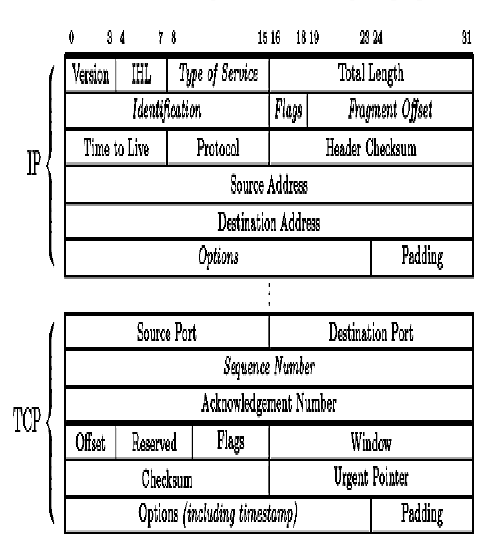
\includegraphics[width=0.5\textwidth]{Basic-TCP-IP-header-structure.png}
				\caption{TCP and IP header packet structure}
			\end{figure}
		\end{column}
		\begin{column}{0.5\textwidth}
			\begin{itemize}
				\item 1980 - TCP/IP stack was implemented on
					Berkeley UNIX
					\pause
				\item Unix people meet ARPANET people. They get
					along really well. The hackers learn C,
					and Unix people learn Networking. Their
					philosophies and approaches are
					remarkably similar, and they blend into
					a single community
			\end{itemize}
		\end{column}
	\end{columns}
\end{frame}

\begin{frame}{TCP/IP and Free Software}
	\begin{columns}
		\begin{column}{0.5\textwidth}
			\begin{figure}
				\centering
				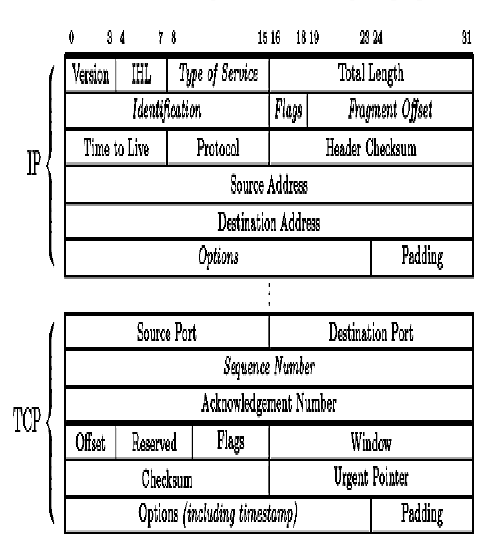
\includegraphics[width=0.5\textwidth]{Basic-TCP-IP-header-structure.png}
				\caption{TCP and IP header packet structure}
			\end{figure}
		\end{column}
		\begin{column}{0.5\textwidth}
			\begin{itemize}
				\item 1981 - Bill Gates makes deal with IBM to
					market MS-DOS independently of the
					hardware it is developed on
					Meanwhile...A Dragon, wise to the game,
					begins to slowly secure a monopoly on
					desktop computing.
					\pause
				\item 1983 - Antitrust case against Bell Labs
					won, and AT\&T can now turn Unix into a
					product Proprietary lock-ins fragment
					cross-platform compatibility: ‘The Unix
					Wars’ AT\&T System V Unix vs BSD Unix
					(No Linux yet).
			\end{itemize}
		\end{column}
	\end{columns}
\end{frame}

\begin{frame}{TCP/IP and Free Software}
	\begin{columns}
		\begin{column}{0.5\textwidth}
			\begin{figure}
				\centering
				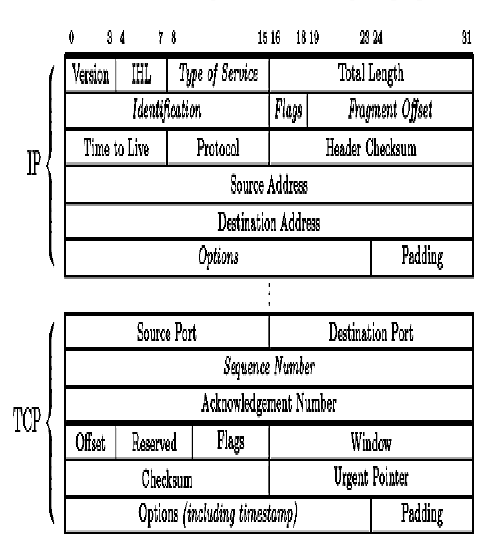
\includegraphics[width=0.5\textwidth]{Basic-TCP-IP-header-structure.png}
				\caption{TCP and IP header packet structure}
			\end{figure}
		\end{column}
		\begin{column}{0.5\textwidth}
			\begin{itemize}
				\item 1985 - GNU Manifesto and the GPL. No
					Linux kernel yet. Stallman defined
					‘hacker culture’, and not everyone was
					okay with him saying exactly what is
					was and wasn’t. The GPL provided legal
					protections to IP. The 4 Freedoms, and
					every derivative gets them.
			\end{itemize}
		\end{column}
	\end{columns}
\end{frame}

\begin{frame}{TCP/IP and Free Software}
	\begin{columns}
		\begin{column}{0.5\textwidth}
			\begin{figure}
				\centering
				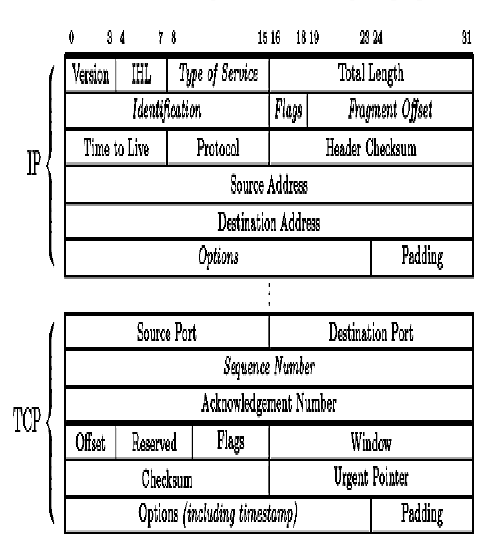
\includegraphics[width=0.5\textwidth]{Basic-TCP-IP-header-structure.png}
				\caption{TCP and IP header packet structure}
			\end{figure}
		\end{column}
		\begin{column}{0.5\textwidth}
			\begin{itemize}
				\item 1988 - POSIX standard Unites Unix and BSD
					The Unix Wars, part II Meanwhile,
					Microsoft is killing it in home and
					small business computers AT\&T and BSD
					eventually settle out of court in 1992,
					but this slowed development at a
					crucial point. The world had decided to
					build the Internet on GNU/Linux.
			\end{itemize}
		\end{column}
	\end{columns}
\end{frame}

\section{Linux and Open Source}
\subsection{1991-200s}
\begin{frame}{Linux and Open Source}
	\begin{columns}
		\begin{column}{0.5\textwidth}
			\begin{figure}
				\centering
				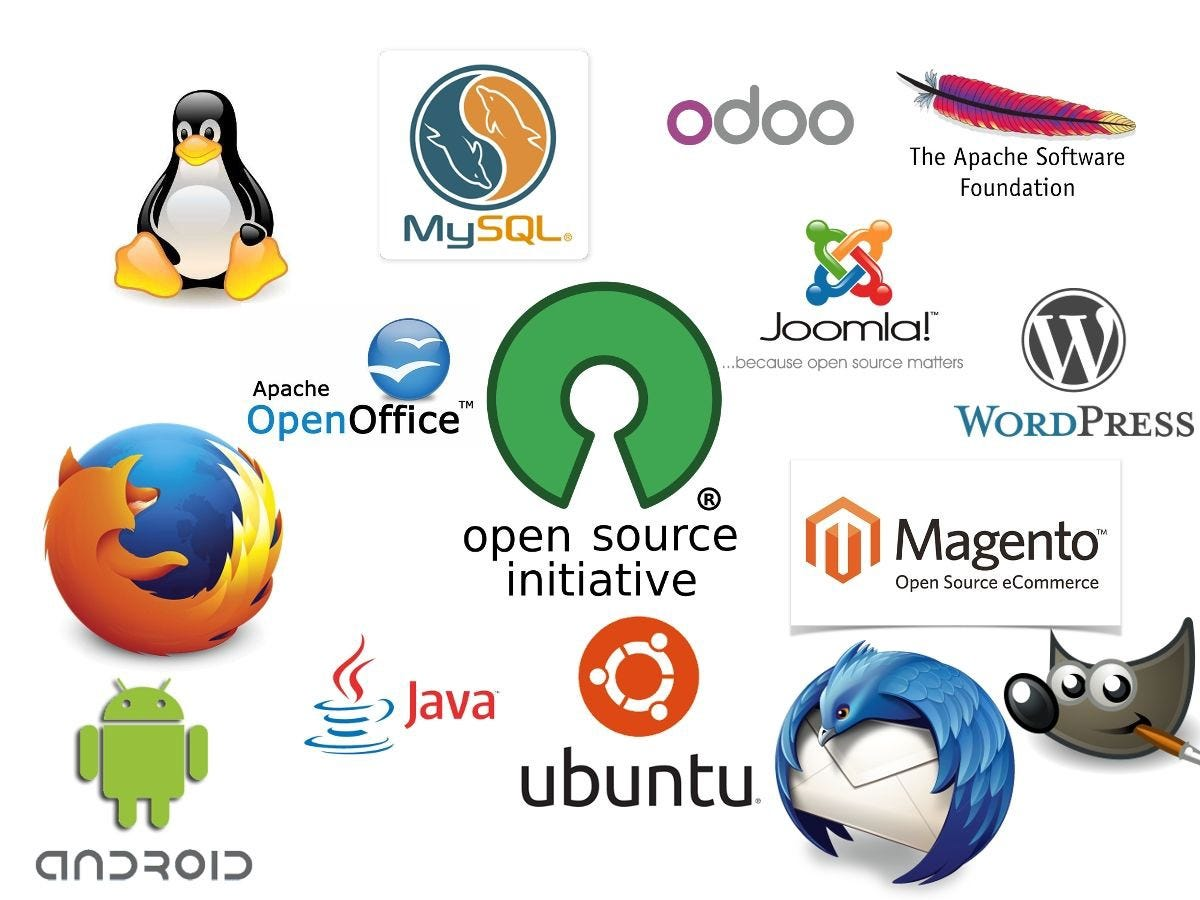
\includegraphics[width=\textwidth]{1_44UXHdH0lxIvxWRvlMId-g.jpg}
			\end{figure}
		\end{column}
		\begin{column}{0.5\textwidth}
			\begin{itemize}
				\item 1993 - Linux has native X and Internet
					\pause
				\item Internet Boom
					\pause
				\item 1995 - Apache
					\pause
				\item Datacenters began to fill with Linux
					machines
					\pause
				\item 1998 - Mozilla Browser and ‘Open source’
					\pause
				\item A large number of Internet and
					free-software groups met and decided to
					change they way they present their
					ethos of information sharing to the
					world Less confrontational, more
					business-friendly
			\end{itemize}
		\end{column}
	\end{columns}
\end{frame}

\begin{frame}{Closing Remarks}
	\begin{center}
		\Huge Thank you!
	\end{center}
\end{frame}

\begin{frame}{Closing Remarks}
	\begin{columns}
		\begin{column}{0.5\textwidth}
			\textbf{Officers}
			\begin{figure}
				\centering
				\includegraphics[width=0.60\textwidth]{officers.png}
			\end{figure}
		\end{column}
		\begin{column}{0.5\textwidth}
			The information in this presentation will be made
			available\footnotemark on our website!\\
			\url{https://lug.cs.uic.edu}
			
			\bigskip
			Join our Discord!

			\begin{figure}
				\centering
				\includesvg[width=0.5\textwidth]{lug-discord.svg}
				\caption{\url{https://discord.gg/NgxTR7PX5e}}
			\end{figure}
		\end{column}
	\end{columns}

	\footnotetext{sooner or later}
\end{frame}

\end{document}

% vim: set tw=80 ts=4 sw
